\subsubsection{Dynamiske side af analysen}
Figure \ref{fig:OpretSag} til \ref{fig:ASOpret} viser hvad gruppen havde tænkt der skal ske i systemmet i første iteration. \\

\begin{figure}[hb]
  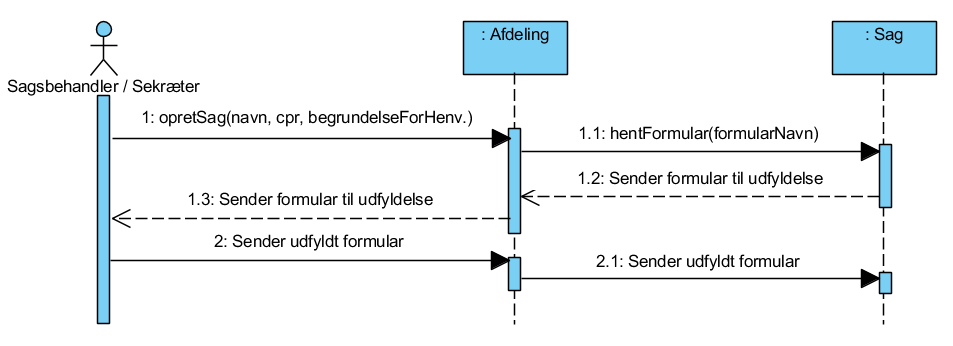
\includegraphics[width=\linewidth]{./PNG/sekDiaOpretSag.PNG} 
  \caption{Sekvensdiagram for opret sag.}
  \label{fig:OpretSag}
\end{figure}

\begin{figure}[hb]
  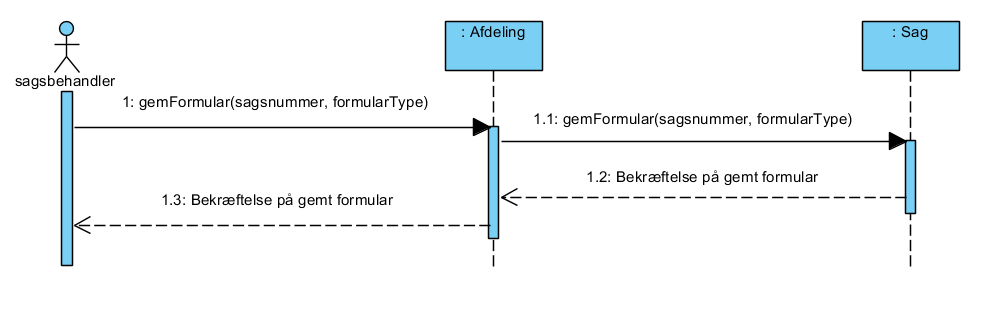
\includegraphics[width=\linewidth]{./PNG/sekDiaGemFormular.PNG} 
  \caption{Sekvensdiagram for gem formular.}
  \label{fig:GemForm}
\end{figure}

\begin{figure}[hb]
  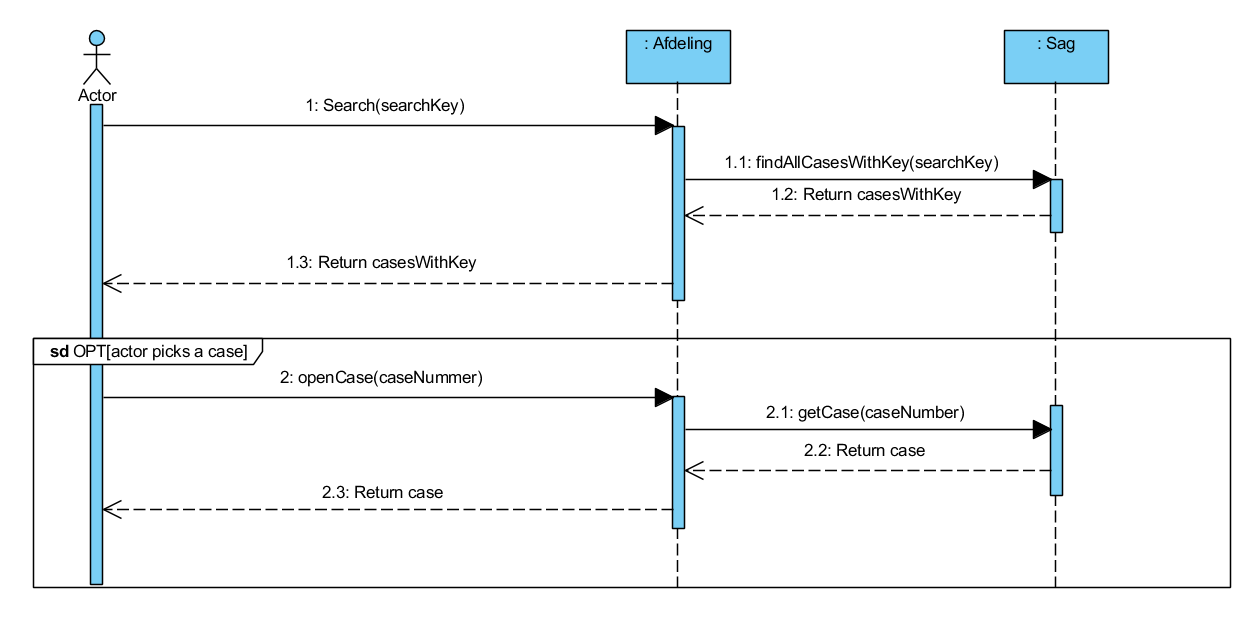
\includegraphics[width=\linewidth]{./PNG/sekDiaFindSag.PNG} 
  \caption{Sekvensdiagram for find sag.}
  \label{fig:FindSag}
\end{figure}

\begin{figure}
  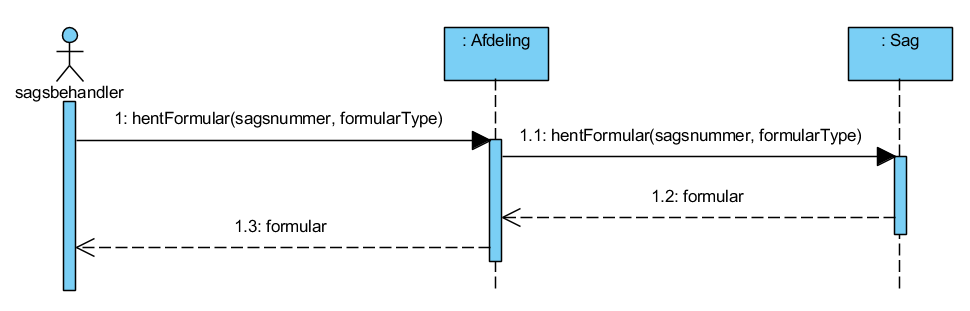
\includegraphics[width=\linewidth]{./PNG/sekDiaHentFormular.PNG} 
  \caption{Sekvensdiagram for hent formular .}
  \label{fig:HentForm}
\end{figure}

\begin{figure}
  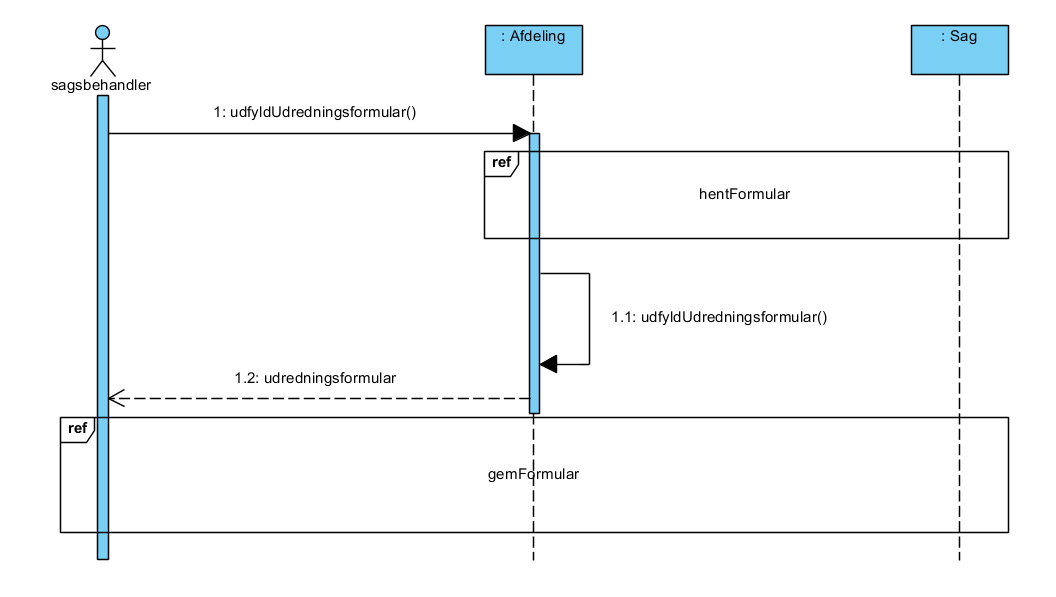
\includegraphics[width=\linewidth]{./PNG/sekDiaUdfyldUdredningsFormular.PNG} 
  \caption{Sekvensdiagram for udfyldning af udrednings formular.}
  \label{fig:UdForm}
\end{figure}

\begin{figure}
  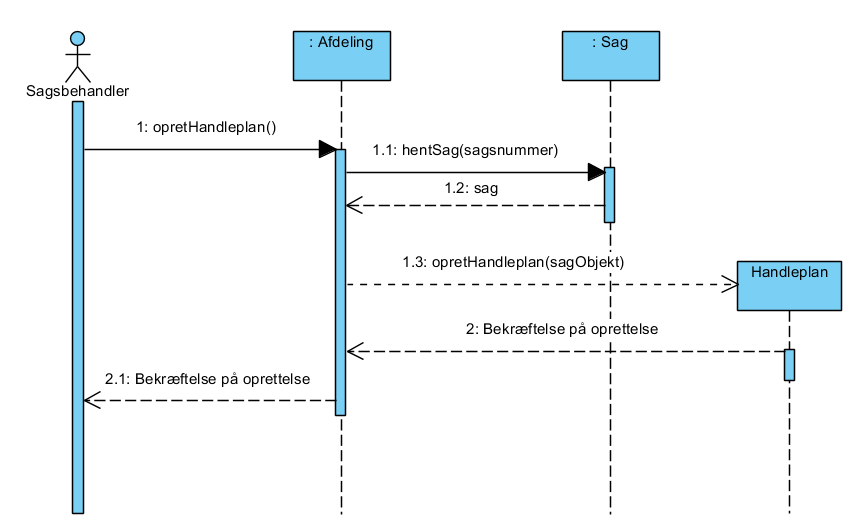
\includegraphics[width=\linewidth]{./PNG/sekDiaOpretHandleplan.PNG} 
  \caption{Sekvensdiagram for opret handleplanen .}
  \label{fig:OpretPlan}
\end{figure}

\begin{figure}
  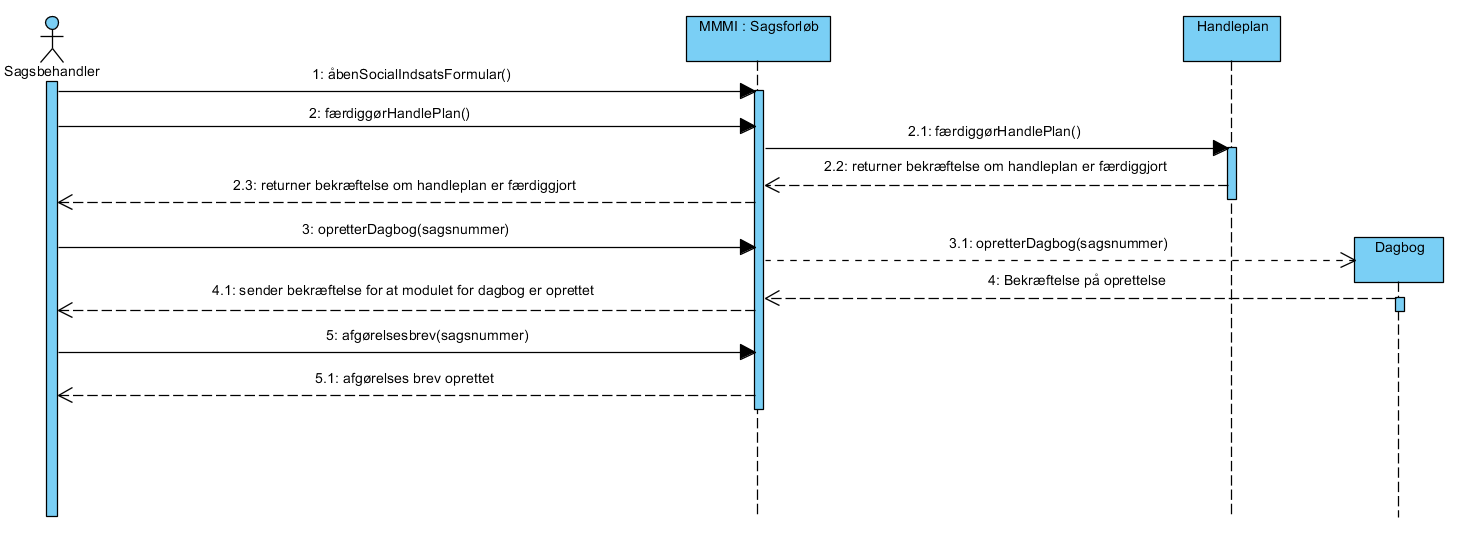
\includegraphics[width=\linewidth]{./PNG/sekDiaSagsforloebAfgoere.PNG} 
  \caption{Sekvensdiagram for opret handleplanen .}
  \label{fig:SagforAf}
\end{figure}

\begin{figure}
  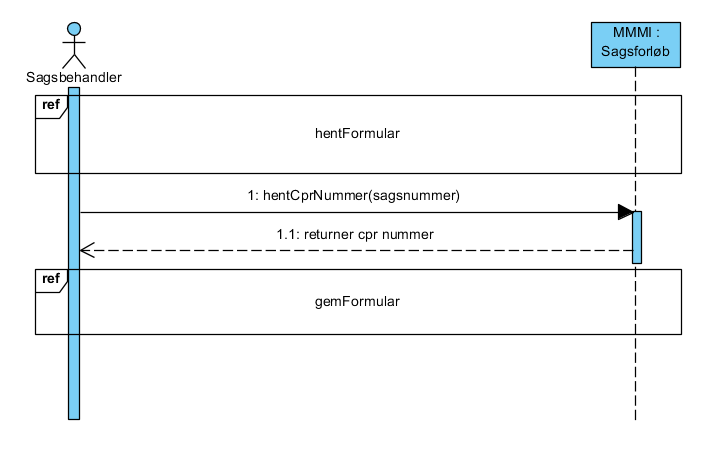
\includegraphics[width=\linewidth]{./PNG/sekDiaSagsforloebIndhent.PNG} 
  \caption{Sekvensdiagram for opret handleplanen .}
  \label{fig:SagforInd}
\end{figure}

\begin{figure}
  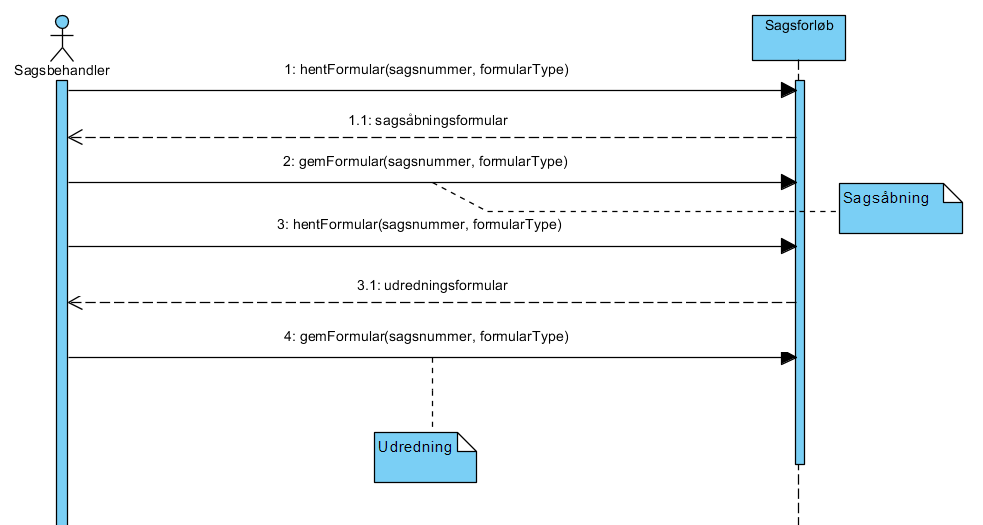
\includegraphics[width=\linewidth]{./PNG/sekDiaBehandelSag.PNG} 
  \caption{Sekvensdiagram for behandel sag.}
  \label{fig:SagforInd}
\end{figure}

\begin{figure}
  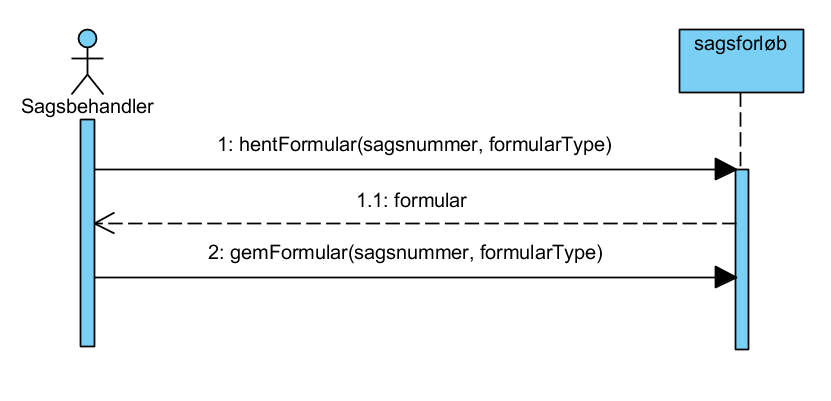
\includegraphics[width=\linewidth]{./PNG/sekDiaBehandelSagMangel.PNG} 
  \caption{Sekvensdiagram for behandel sag hvor der er mangel på information.}
  \label{fig:BSMangel}
\end{figure}

\begin{figure}
  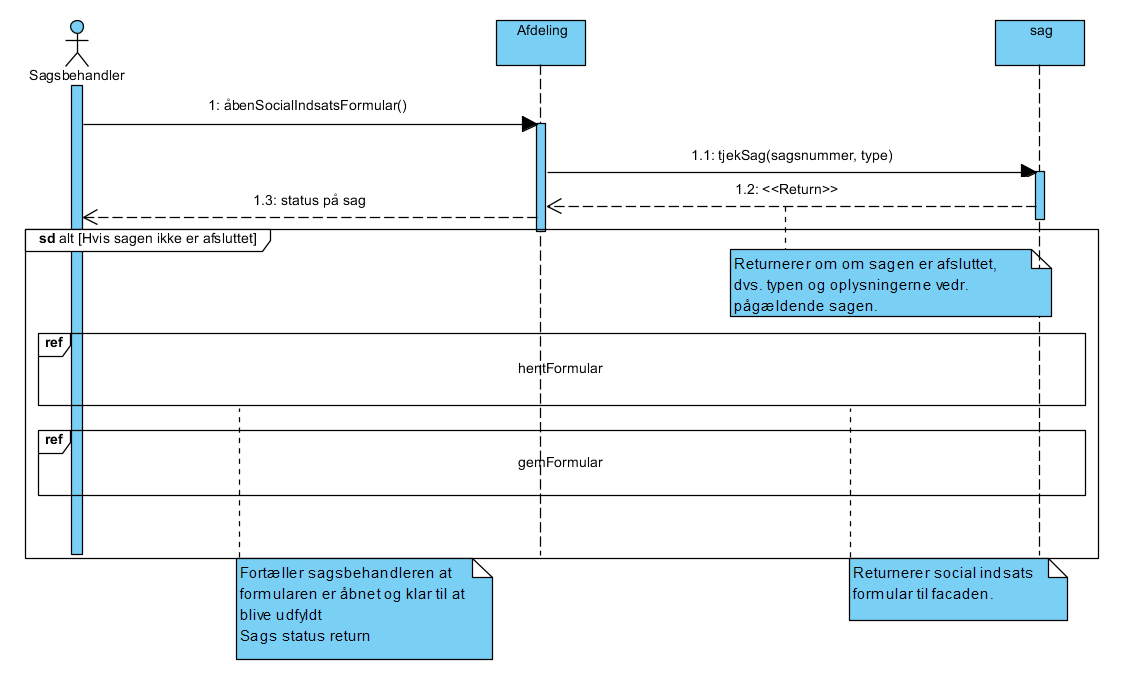
\includegraphics[width=\linewidth]{./PNG/sekDiaAfgoereSagsbehandaaben.PNG} 
  \caption{Sekvensdiagram for behandel sag hvor der er mangel på information.}
  \label{fig:ASAA}
\end{figure}


\begin{figure}
  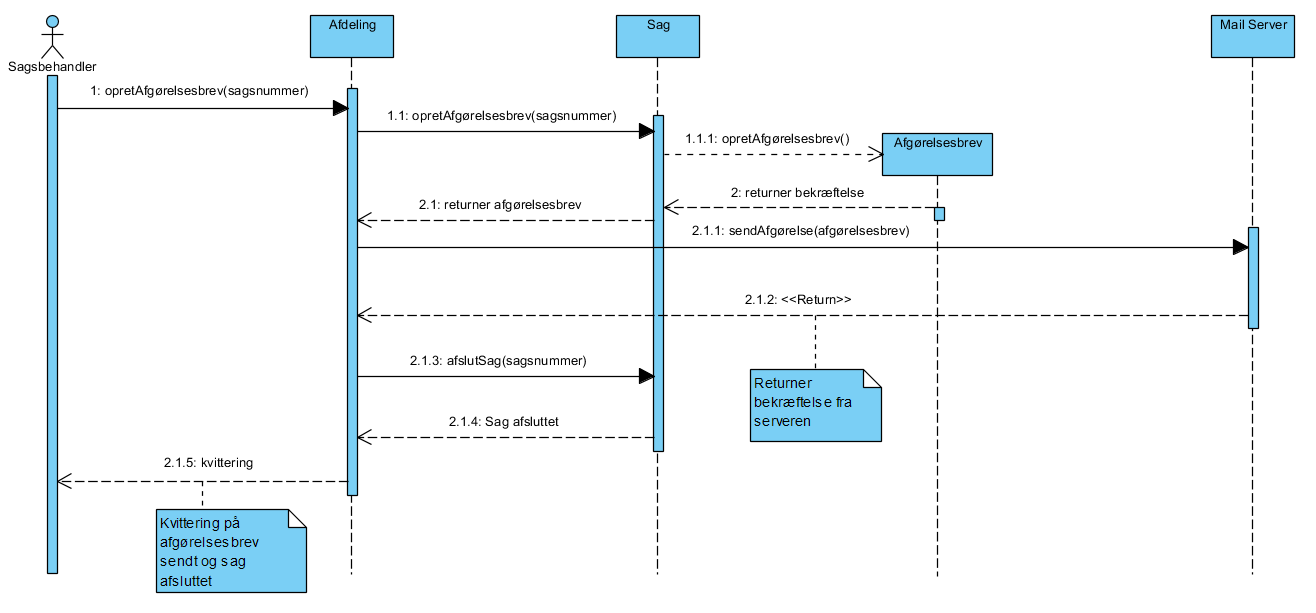
\includegraphics[width=\linewidth]{./PNG/sekDiaAfgoereSagsbehandAfgoerelse.PNG} 
  \caption{Sekvensdiagram for behandel sag hvor der er mangel på information.}
  \label{fig:ASAf}
\end{figure}

\begin{figure}
  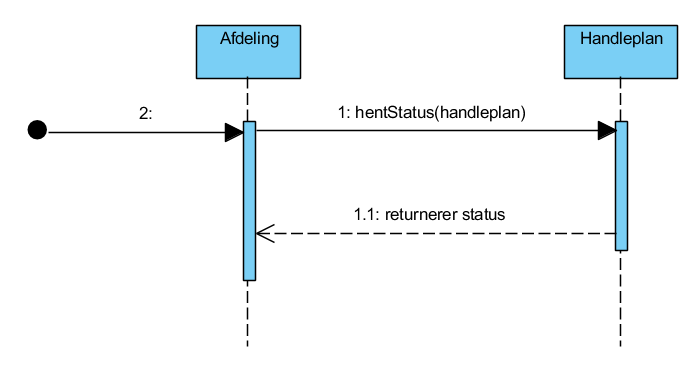
\includegraphics[width=\linewidth]{./PNG/sekDiaAfgoereSagsbehandFaerdig.PNG} 
  \caption{Sekvensdiagram for behandel sag hvor der er mangel på information.}
  \label{fig:ASFaer}
\end{figure}

\begin{figure}
  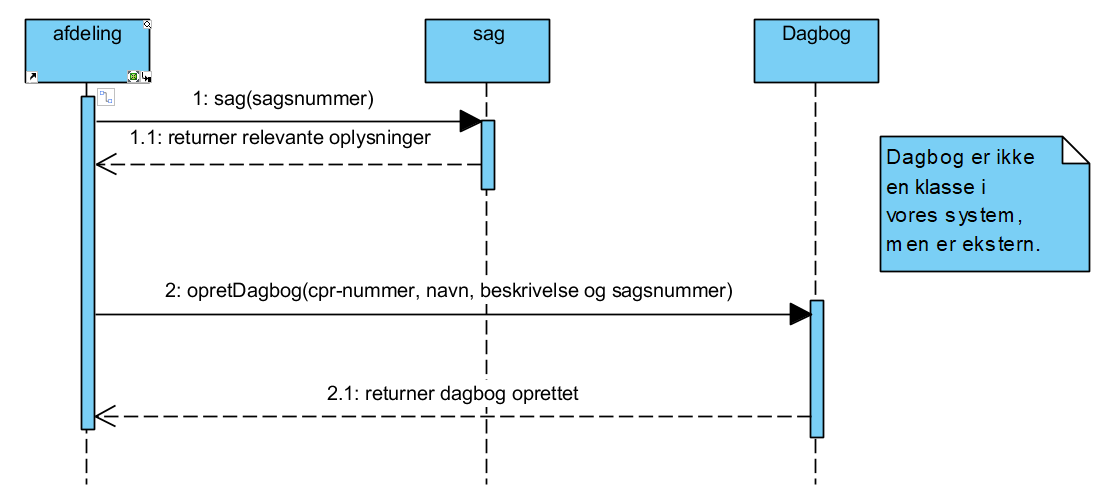
\includegraphics[width=\linewidth]{./PNG/sekDiaAfgoereSagsbehandOpret.PNG} 
  \caption{Sekvensdiagram for behandel sag hvor der er mangel på information.}
  \label{fig:ASOpret}
\end{figure}
